\documentclass[border=10pt]{standalone}
\usepackage{tikz}\usepackage{amsmath}\usetikzlibrary{arrows.meta,decorations.markings}
\begin{document}
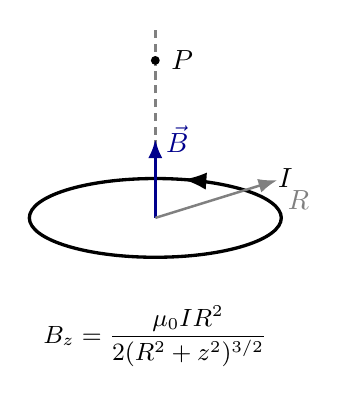
\begin{tikzpicture}[line width=0.9pt,>={Latex[length=2.4mm]}]
  \draw[line width=1.2pt,decoration={markings,mark=at position 0.2 with {\arrow{Latex}}},postaction={decorate}] (0,0) ellipse (1.6 and 0.5);
  \node at (1.65,0.5){$I$};
  \draw[densely dashed,gray] (0,0)--(0,2.4);
  \fill (0,2.0) circle(1.6pt) node[right=2pt]{$P$};
  \draw[->,blue!55!black,line width=1.2pt] (0,0)--(0,1.0) node[right]{$\vec B$};
  \draw[->,gray] (0,0)--(1.55,0.48) node[below right]{$R$};
  \node at (0,-1.5){\small $\displaystyle B_z=\frac{\mu_0 I R^2}{2(R^2+z^2)^{3/2}}$};
\end{tikzpicture}
\end{document}
